\chapter{\MakeUppercase{Methodology and Testing}}

\section{Experimental Methodology}
The design used in this study is one which strikes a balance between these two techniques. Even as the chosen design utilizes the simplicity of contact-based algorithmic routing, it has enough information to aid in decision-making. What makes this very important is the fact that choosing a too simplistic technique will make us miss out on an invaluable chance in terms of disaster management.

\section{Experimental Controls and Fairness}
Methodology has been defined in such a way that a fair comparison could be ensured. In this regard, all protocols have been analyzed using similar conditions, such as disaster region, set of nodes, mobility model, buffer size, TTL of message, and probabilities for sending traffic. It is also noted that the router proposed in this work can make use of its locally maintained state, and not the external oracle.

Protocol results from the test run also remain consistent. Deliveries, delays, overheads, and drops are all calculated using the same counters irrespective of the router chosen. Aggregation of the results is conducted after multiple runs to avoid any influence of randomness due to node movements and messaging on the results. The intent is to compare routing strategies, not isolated lucky or unlucky runs.

\section{Traffic Scenarios}
The traffic scenarios are defined by per-node message generation probability:

\begin{table}[h!]
	\centering
	\caption{Traffic scenarios}
	\renewcommand{\arraystretch}{1.3}
	\begin{tabular}{|l|l|l|}
		\hline
		\textbf{Traffic Level} & \textbf{Generation Probability} & \textbf{Interpretation} \\
		\hline
		Low & 3/3600 & Light background communication \\
		\hline
		Medium & 8/3600 & Moderate disaster coordination traffic \\
		\hline
		High & 20/3600 & Congested emergency communication \\
		\hline
	\end{tabular}
	\label{tab:traffic_scenarios}
\end{table}

\section{Baseline Protocol Testing}
Epidemic routing is tested to measure the behavior of unrestricted replication. It forwards every message to every encountered node that does not already have it, provided the receiver buffer has space. This baseline helps show the cost of blind reachability.

Spray and Wait routing is tested to measure copy-limited forwarding. The implementation gives one copy at a time during the spray phase and forwards a single-copy message only when the destination is encountered. This baseline helps show the cost of conservative forwarding.

\section{Proposed Protocol Testing}
Spatio-Semantic routing is tested using the same traffic and mobility conditions. Its main test objective is to determine whether spatial, semantic, and priority-aware decisions improve performance under load. The protocol is expected to be especially strong when traffic is high because congestion exposes whether buffer and relay choices are meaningful.

In addition to aggregate performance, the proposed protocol is interpreted in relation to its design claims. If the critical buffer reserve is useful, critical delivery should degrade more slowly than in the flooding baseline as traffic increases. If semantic and spatial relay selection are useful, average critical delay should improve compared with Spray and Wait, especially once simple waiting becomes costly. These expectations provide a more detailed basis for reading the results than a single overall winner/loser comparison.

\section{Dashboard and Visual Testing}
The project includes a Streamlit dashboard for plotting metric trends, radar comparisons, raw results, and launching the live visual simulation. The live visualizer compares the three protocols side by side with the same initial seed and displays delivery, critical delivery, critical delay, overhead, drops, contacts, node roles, and critical-message carriers.

The dashboard plots themselves are used to support interpretation of the quantitative findings, so they are discussed alongside the corresponding analysis in the results chapter rather than being grouped here as a separate gallery. In this chapter, the more relevant visual evidence is the live validation interface used during testing.

\begin{figure}[h!]
    \centering
    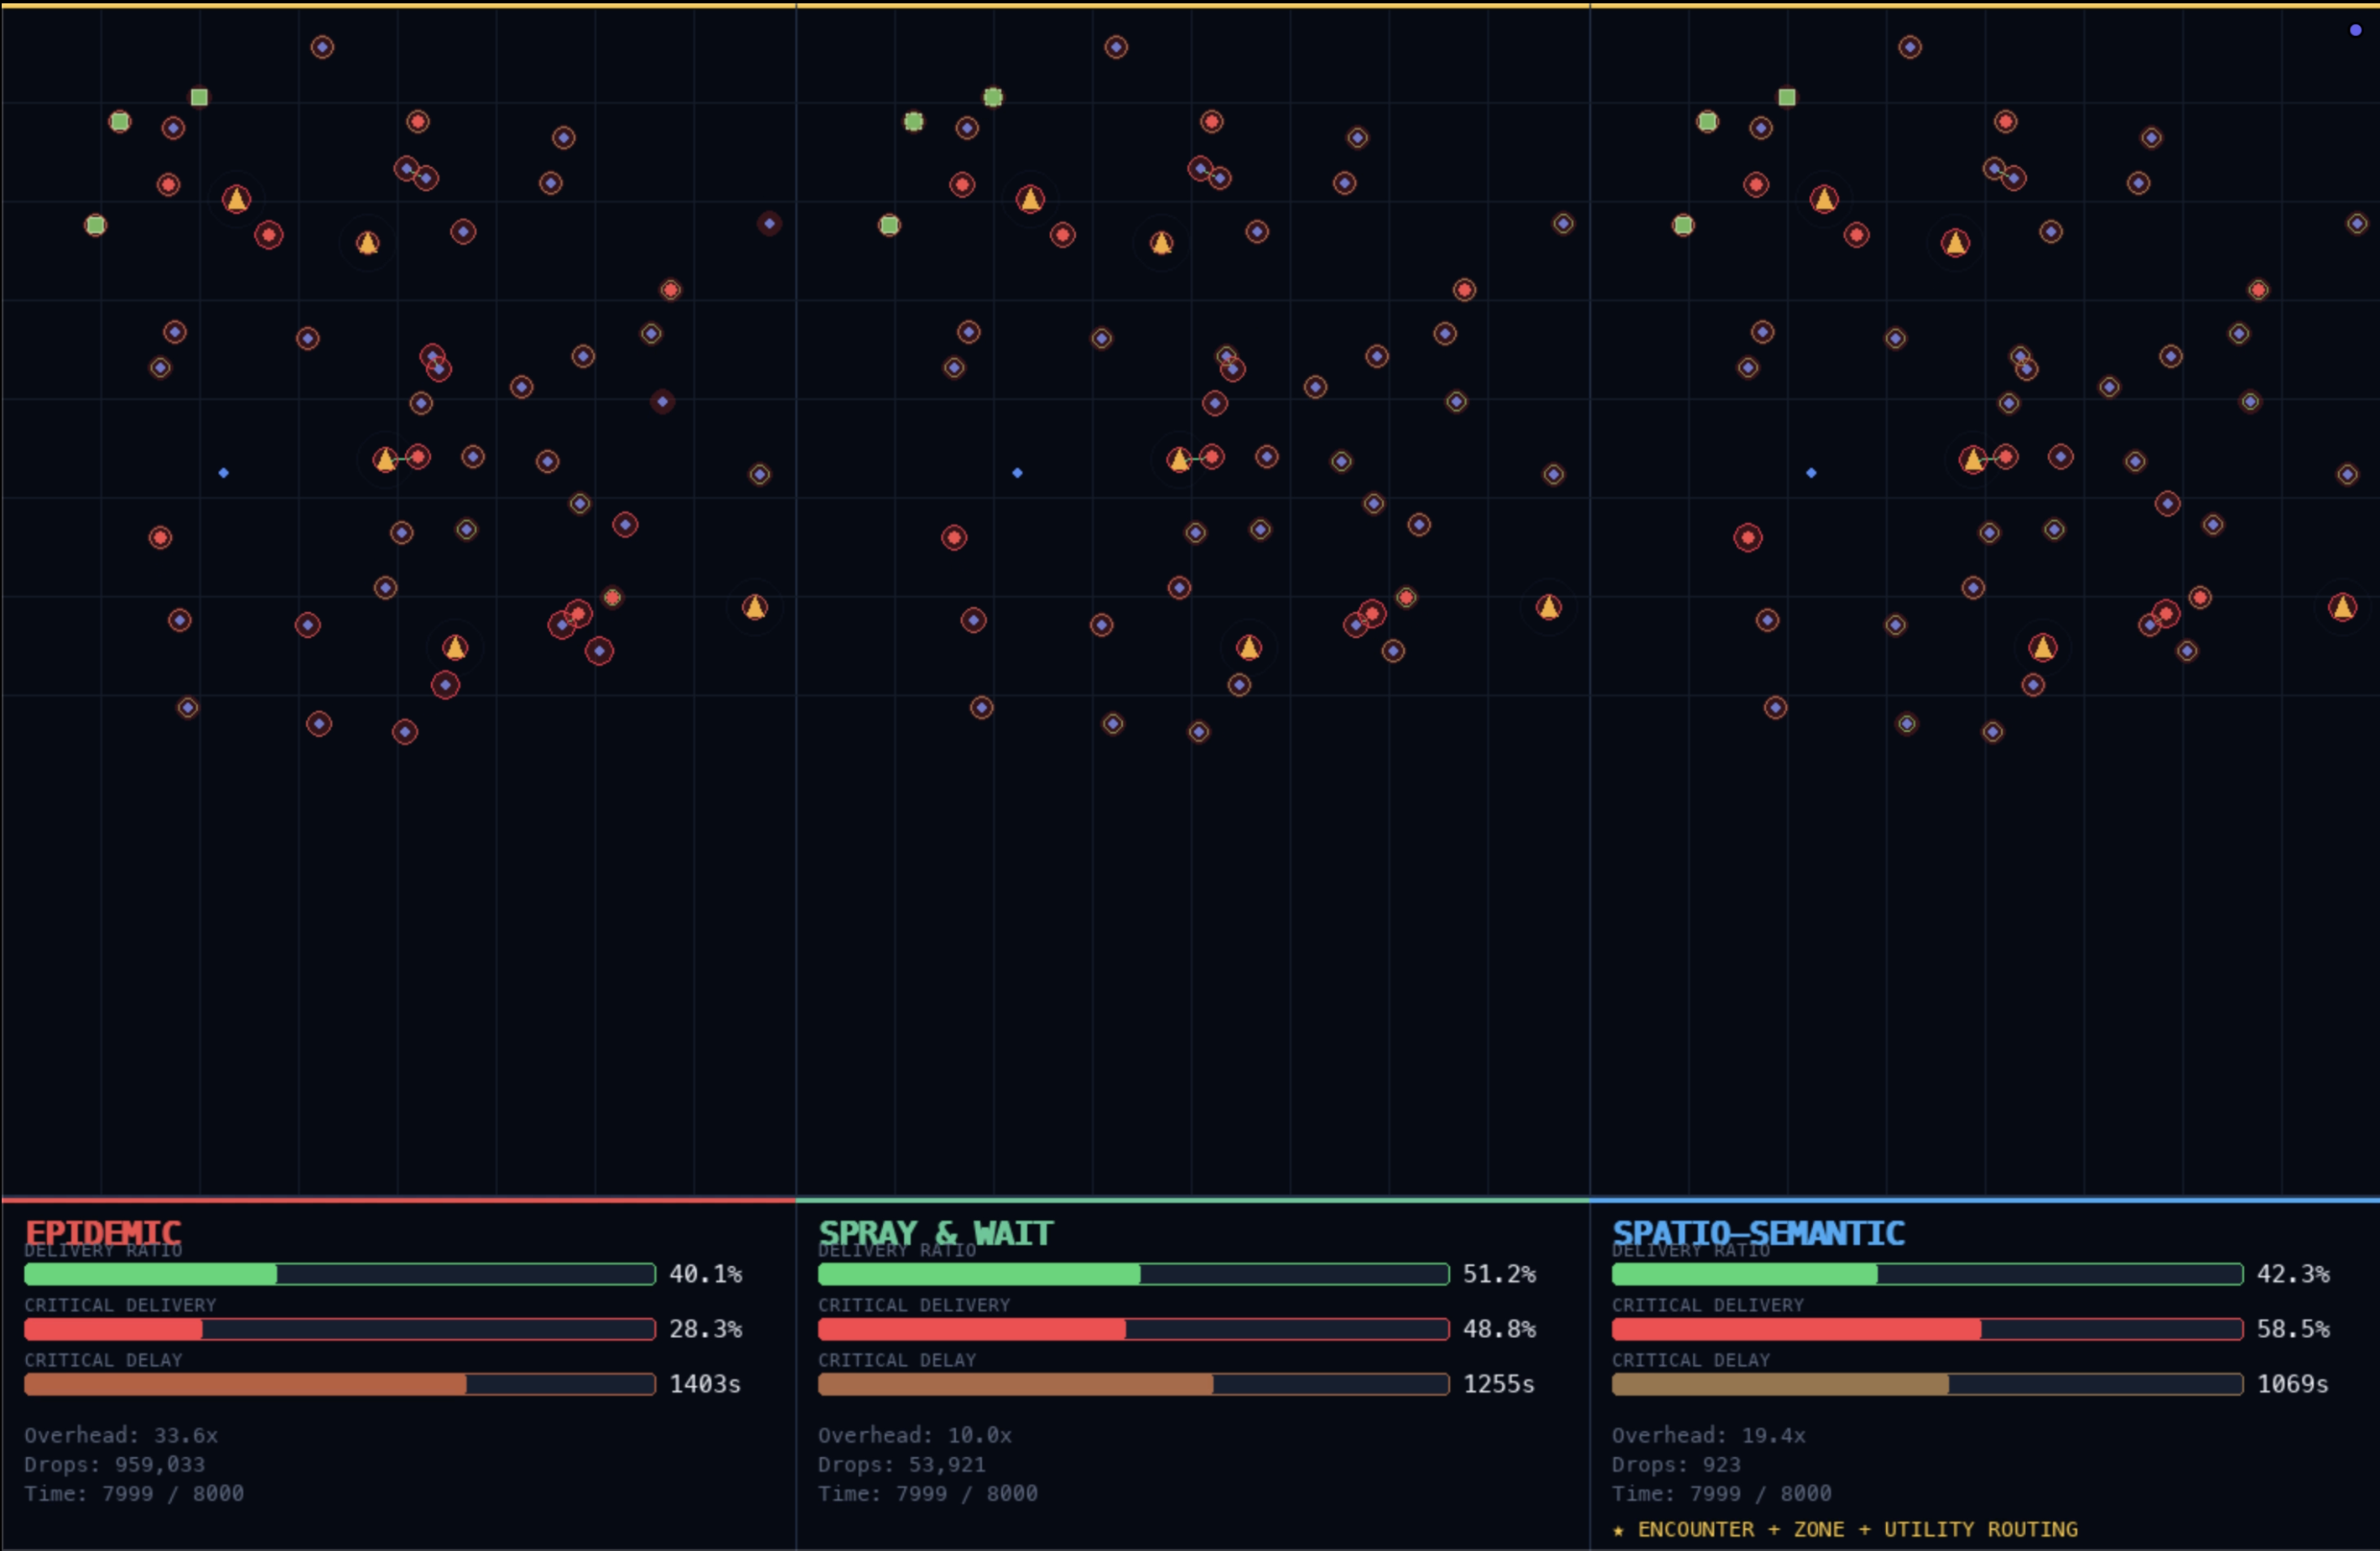
\includegraphics[width=0.85\textwidth]{images/demo-ss.png}
    \caption{Live three-panel simulation of competing DTN routing protocols}
    \label{fig:live_sim_placeholder}
\end{figure}

The live comparison is useful because it exposes how protocol behavior emerges over time. During testing, it allows direct inspection of contact opportunities, carrier movement, congestion build-up, and the treatment of critical traffic. This makes it easier to verify that the measured metrics are consistent with the underlying routing behavior before the formal results are interpreted.

\section{Testing Criteria}
The protocol is considered successful if it satisfies the following criteria:

\begin{itemize}
	\item It should match or exceed Epidemic routing in delivery under light and medium traffic without increasing congestion unnecessarily.
	\item It should significantly outperform Epidemic routing under high traffic, where flooding is expected to collapse.
	\item It should have a shorter critical-message-delay time than Spray and Wait since an emergency message cannot be held back until it is delivered directly.
	\item Under congested conditions, it should still enjoy superiority in terms of critical delivery ratio.
\end{itemize}

\section{Reproducibility and Validity Considerations}
The reason for running each scenario twenty times is that the impact of any individual mobility trace or contact profile will be reduced, which improves the accuracy of the results obtained. This is especially relevant for \acp{dtn}, as small differences at the beginning might affect the entire process of dissemination of messages.

Nevertheless, there are some limitations regarding the validity of these results that need to be considered. First, the model of random waypoints is not suitable for representing all types of movement of disasters. Second, the simulation of the wireless network fails to take into account interference, competition for the channel and energy exhaustion. Although it might seem that these limitations undermine the whole study, they actually define its range and boundaries.

\section{Result Interpretation Strategy}
Evaluation is done using both the criteria of absolute measurement and comparative trends. Absolute measurements provide valuable information in that they help understand the actual impact of delivery, latency, overhead, and packet dropping in the presence of each traffic pattern. Equally crucial is comparative trend analysis, which will help us understand the speed at which each protocol breaks down as the level of traffic progresses from light to heavy. Both aspects are taken into consideration by this thesis because a protocol that seems good in one instance can be bad in another.

Specific attention is paid to the protocol’s performance during high traffic, since this case corresponds most closely to the reason behind developing the thesis. During disaster communication, the most critical periods usually occur when the system is heavily loaded and its infrastructure is least robust. As such, a protocol which performs well only when it is lightly loaded is not very convincing in this context. The testing methodology places special focus on evaluating whether the protocol can still be useful in adverse conditions.

\section{Role of Visual Validation}
However, it should be noted that the visual analysis tools are not intended as an alternative to quantitative testing; they simply offer an additional angle on protocol performance. Graphs help in discerning the general tendencies depending on the volume of traffic, whereas live simulations help in understanding the dynamics of how those tendencies arise based on contact chances, buffer loads, and relays' location on the map. In the case of \acp{dtn}, protocol dynamics are highly influenced by the physical separation between nodes and their occasional contacts.

Graphical validation is also useful in revealing unexpected behaviors. For instance, although the protocol demonstrates satisfactory overall packet delivery rate, there might still be noticeable congestion at particular node types or map areas.
